%%%%%%%%%%%%%%%%%%%%%%%%%%%%%%%%%%%%%%%%%
% Short Sectioned Assignment
% LaTeX Template
% Version 1.0 (5/5/12)
%
% This template has been downloaded from:
% http://www.LaTeXTemplates.com
%
% Original author:
% Frits Wenneker (http://www.howtotex.com)
%
% License:
% CC BY-NC-SA 3.0 (http://creativecommons.org/licenses/by-nc-sa/3.0/)
%
%%%%%%%%%%%%%%%%%%%%%%%%%%%%%%%%%%%%%%%%%

%----------------------------------------------------------------------------------------
%	PACKAGES AND OTHER DOCUMENT CONFIGURATIONS
%----------------------------------------------------------------------------------------

\documentclass[paper=a4, fontsize=11pt]{scrartcl} % A4 paper and 11pt font size

\usepackage[T1]{fontenc} % Use 8-bit encoding that has 256 glyphs
\usepackage{fourier} % Use the Adobe Utopia font for the document - comment this line to return to the LaTeX default
\usepackage[english]{babel} % English language/hyphenation
\usepackage{amsmath,amsfonts,amsthm} % Math packages

\usepackage{lipsum} % Used for inserting dummy 'Lorem ipsum' text into the template

\usepackage{sectsty} % Allows customizing section commands
\allsectionsfont{\centering \normalfont\scshape} % Make all sections centered, the default font and small caps

\usepackage{graphicx} %Figures

\usepackage{fancyhdr} % Custom headers and footers
\pagestyle{fancyplain} % Makes all pages in the document conform to the custom headers and footers
\fancyhead{} % No page header - if you want one, create it in the same way as the footers below
\fancyfoot[L]{} % Empty left footer
\fancyfoot[C]{} % Empty center footer
\fancyfoot[R]{\thepage} % Page numbering for right footer
\renewcommand{\headrulewidth}{0pt} % Remove header underlines
\renewcommand{\footrulewidth}{0pt} % Remove footer underlines
\setlength{\headheight}{13.6pt} % Customize the height of the header

\numberwithin{equation}{section} % Number equations within sections (i.e. 1.1, 1.2, 2.1, 2.2 instead of 1, 2, 3, 4)
\numberwithin{figure}{section} % Number figures within sections (i.e. 1.1, 1.2, 2.1, 2.2 instead of 1, 2, 3, 4)
\numberwithin{table}{section} % Number tables within sections (i.e. 1.1, 1.2, 2.1, 2.2 instead of 1, 2, 3, 4)

\setlength\parindent{0pt} % Removes all indentation from paragraphs - comment this line for an assignment with lots of text

%----------------------------------------------------------------------------------------
%	TITLE SECTION
%----------------------------------------------------------------------------------------

\newcommand{\horrule}[1]{\rule{\linewidth}{#1}} % Create horizontal rule command with 1 argument of height

\title{	
\normalfont \normalsize 
\textsc{Aalborg University} \\ [25pt] % Your university, school and/or department name(s)
\horrule{0.5pt} \\[0.4cm] % Thin top horizontal rule
\huge Worksheet - Rules \\ % The assignment title
\horrule{2pt} \\[0.5cm] % Thick bottom horizontal rule
}

\date{\normalsize\today} % Today's date or a custom date

\begin{document}

\maketitle % Print the title

%----------------------------------------------------------------------------------------
%	PROBLEM 1
%----------------------------------------------------------------------------------------

\section{Purpose}

The purpose was to test the system used in the expert review, including hardware load and frame times. This was done to ensure a "smooth" (pls fix) test and to determine whether potential issues could be attributed to physical limitations. Since the review and system test were both performed over LAN, no latency testing was performed.

\subsection{Methods}

The test was performed at AAU's Audio-Visual Arena using the computers described in \autoref{tab:specs}. 

\begin{table}
\centering
\begin{tabularx}{0.48\textwidth}{X X X}
\toprule
                     & \textit{Computer A} & \textit{Computer B} \\ \midrule \rowcolor{lightGrey}
\textbf{CPU}         & Intel Core i7-4770  & Intel Core i7-6700  \\

\textbf{GPU}         & Nvidia GTX 980      & Nvidia GTX 980    \\  \rowcolor{lightGrey}

\textbf{RAM} 		 & 16GB                & 16GB                 \\ \toprule
\end{tabularx}
\caption{Specifications of the computers used}
\label{tab:specs}
\end{table}

Two players and two observers were present. The players moved around in an introduction scene and in the final scene used in the system review. The observers recorded data using MSI Afterburner and Fraps to measure CPU and GPU load as well as framerate.

\subsection{Results}
The results from the hardware monitoring is shown below. The range indicates roughly 10 minutes of play. 

\begin{figure}[H]
\centering
\includegraphics[width=0.9\textwidth]{B_usage.PNG}
\caption{Hardware usage of Computer A}
\end{figure}

\begin{figure}[H]
\centering
\includegraphics[width=0.9\textwidth]{C_gpu.PNG}
\includegraphics[width=0.9\textwidth]{C_cpu.PNG}
\caption{Hardware usage of Computer B}
\end{figure}

The results from recording framerate is shown below.

\begin{figure}[H]
\centering
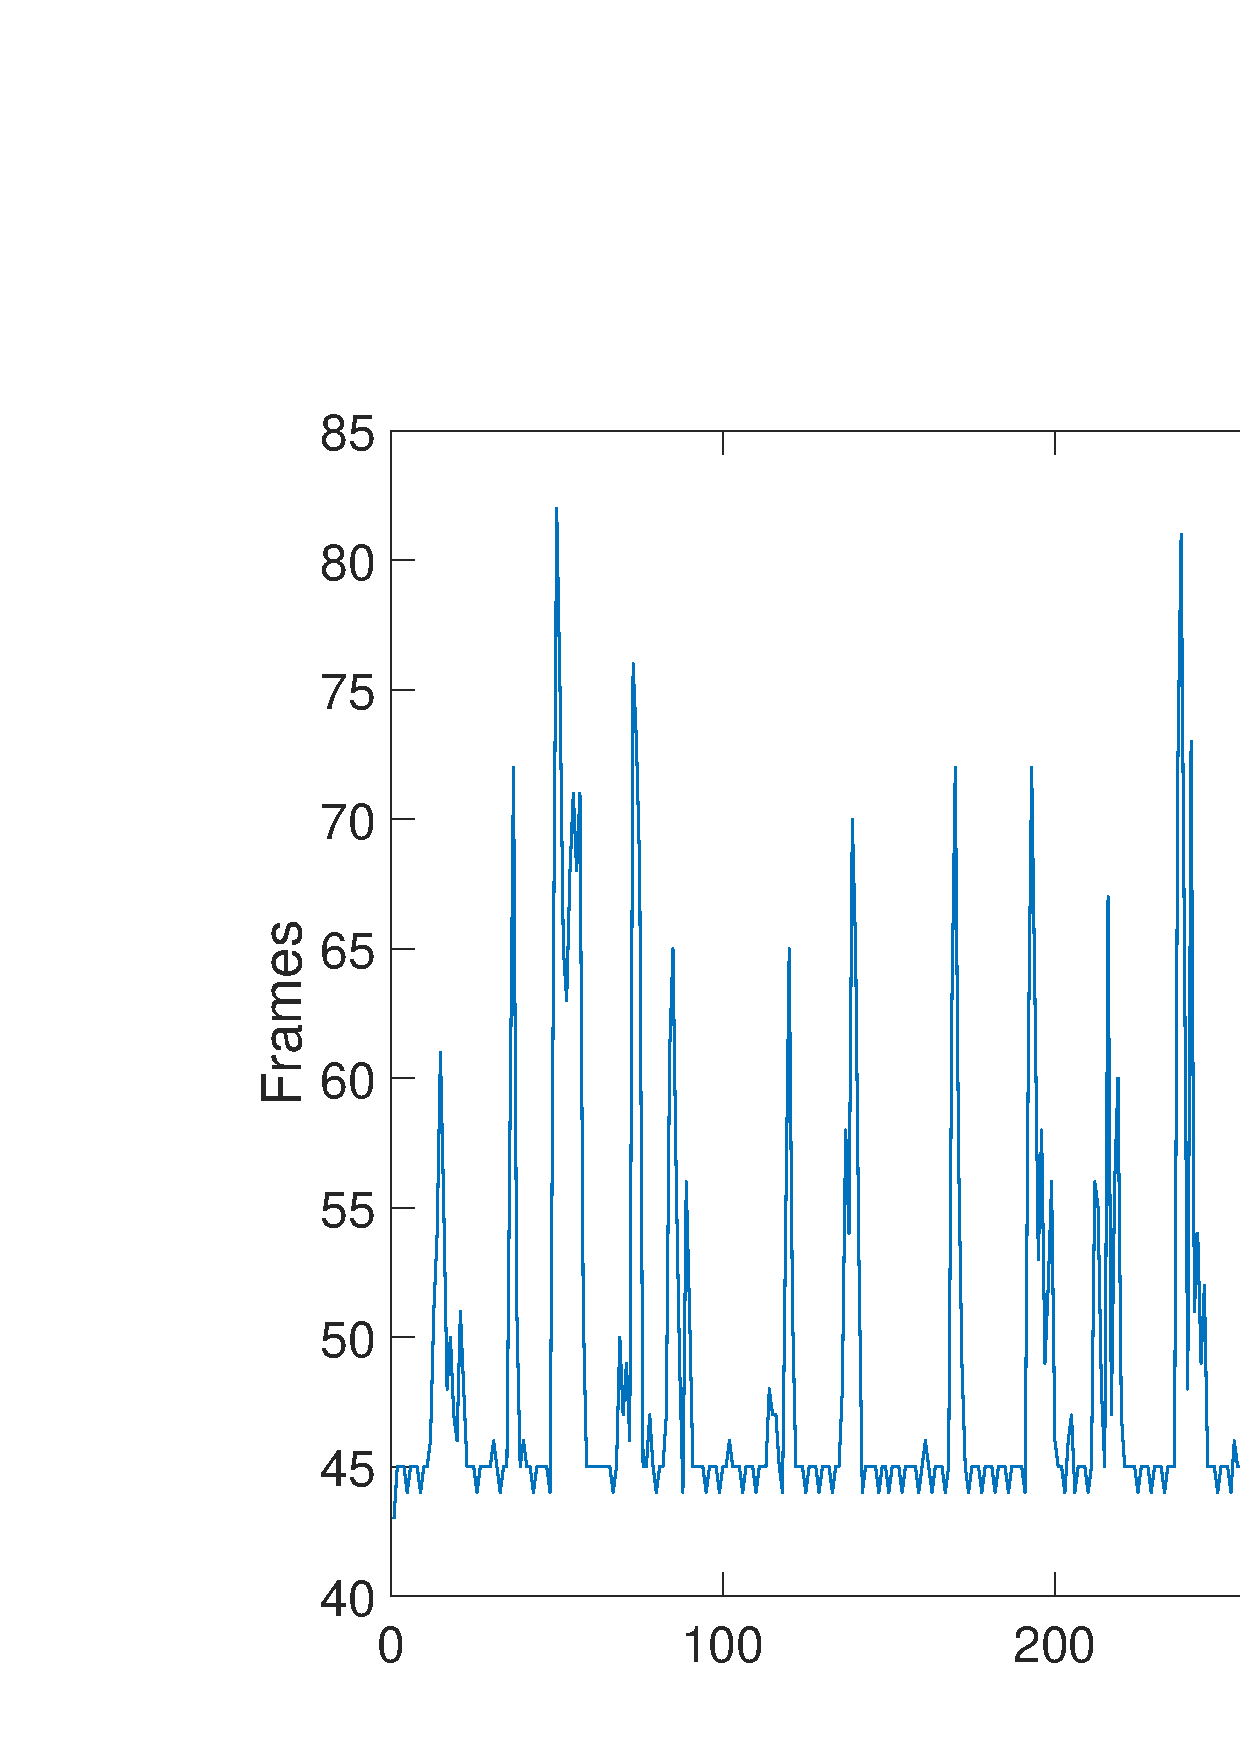
\includegraphics[scale=1]{A_fps.PNG}
\caption{Results from recording framerate in Computer A}
\end{figure}

\begin{figure}[H]
\centering
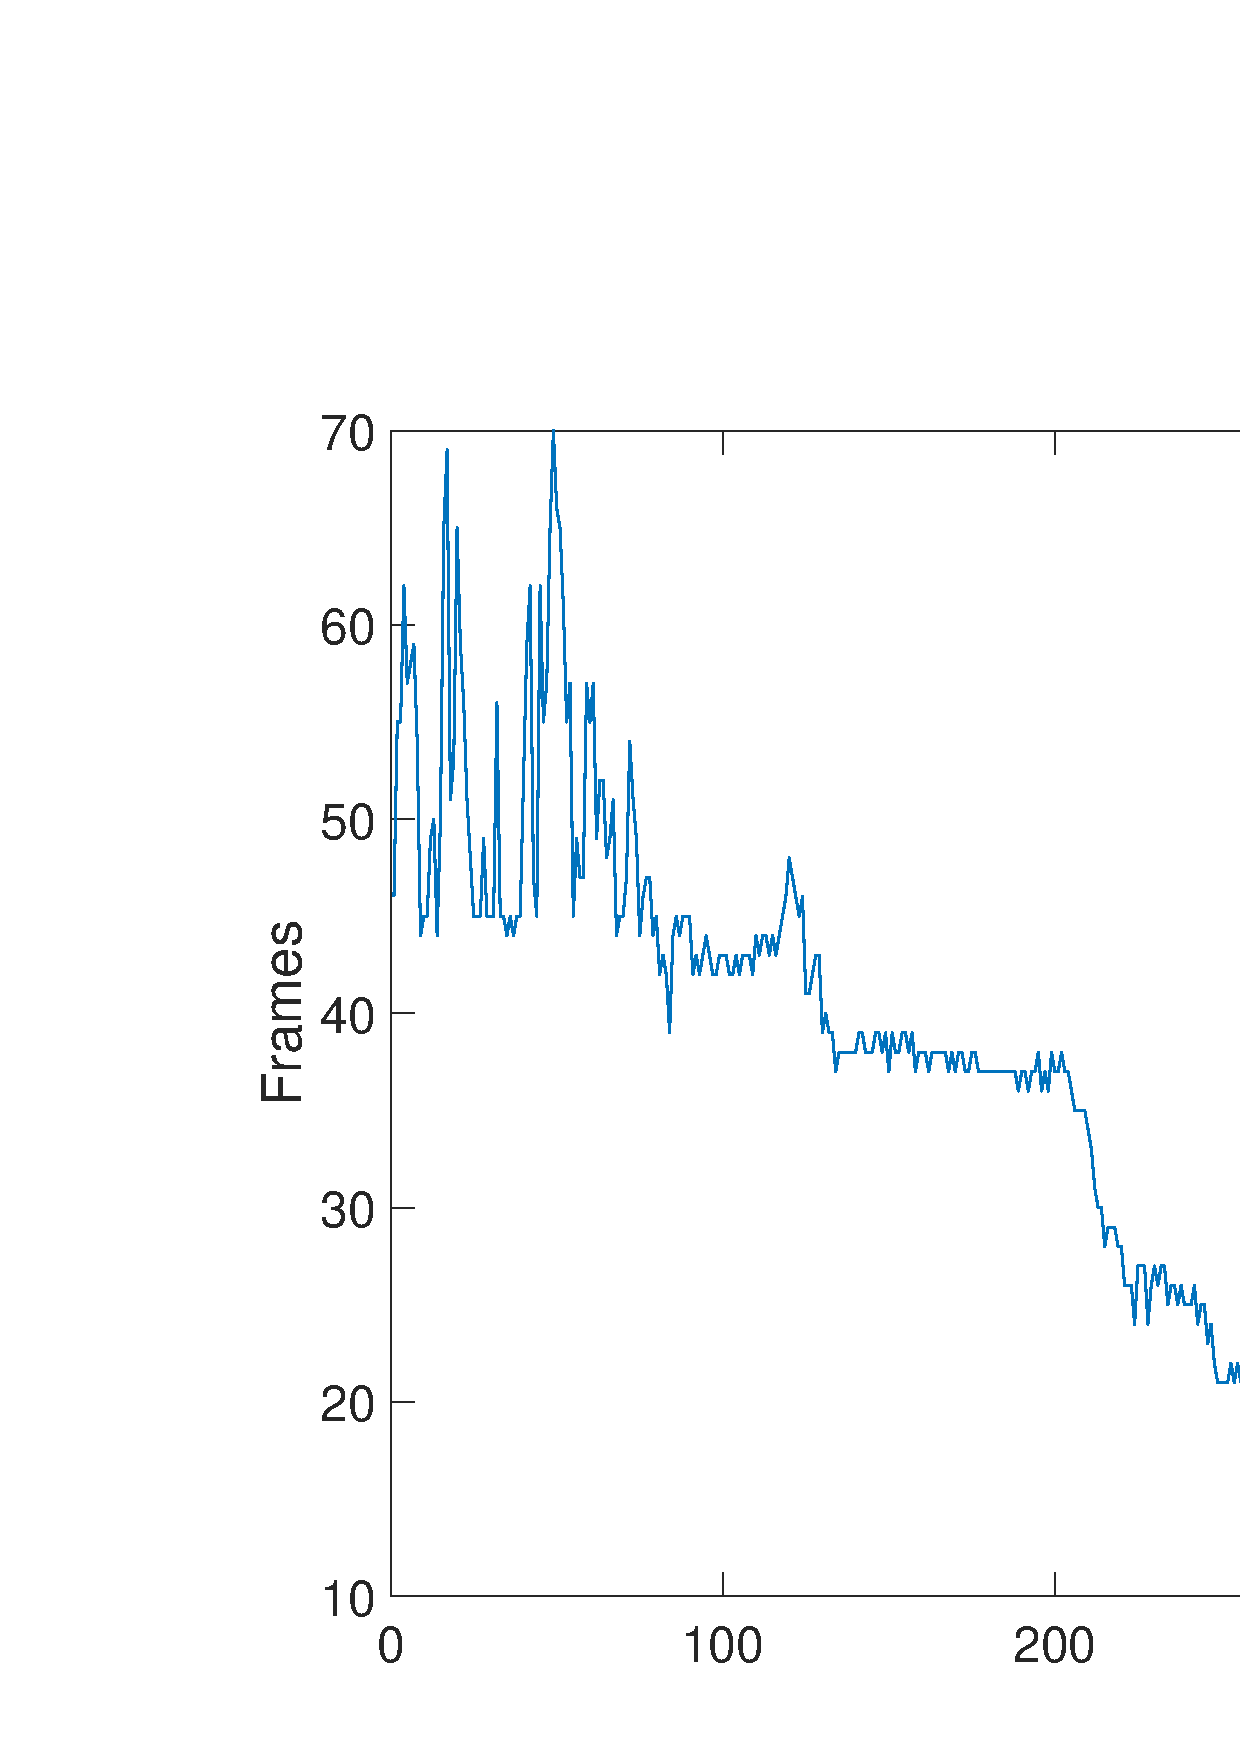
\includegraphics[scale=1]{B_fps.PNG}
\caption{Results from recording framerate in Computer B}
\end{figure}


\subsection{Conclusion}
The framerate results show line at 45 frames per second, however monitoring in the same scene before beginning the recording showed a steady 90 frames per second. We hypothesize that the recording software is at fault, and cannot accurately record framerate in virtual reality applications. This was, however, the only possible solution since no native software can log it. 

The results show a steady decline in framerate for the client computer. This was confirmed in several tests to be the case for any computer used as client, but does not seem to be caused by overheating. The client's GPU usage steadily drops while CPU usage seems to jump. 

This may be the fault of the Proteus multiplayer template for Unreal, and the issue could be writing to a file or otherwise adding data to an array that must be processed at each frame. The issue can be fixed by starting the scene using "25 minutes play time" instead of 10 minutes.

%----------------------------------------------------------------------------------------

\end{document}